% First page
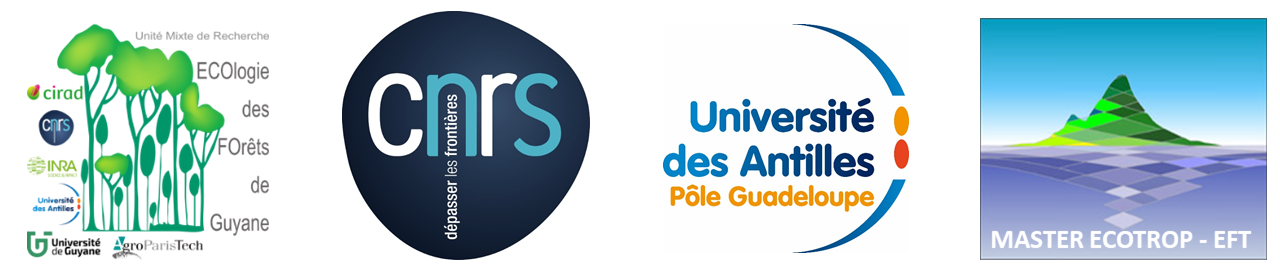
\includegraphics{images/logos}

\begin{center}
\Large{\textbf{Université des Antilles}} \\
  \vspace*{\stretch{1}}
  \LARGE{\textbf{Mémoire de stage}} \\
  \vspace*{\fill}
  \large{présenté par} \\
  \large{Nino PAGE} \\
  \vspace*{\fill}
  \large{pour obtenir le diplôme national de master} \\
  \large{parcours Ecologie des écosystèmes Tropicaux naturels et exploités (ECOTROP)} \\
  \small{spécialité : Ecologie des Forêts Tropicales} \\
  \vspace*{\fill}
  \large{Sujet :} \\
  \Large{\textbf{Modeling the impacts of selective logging on tropical forests: A first attempt with TROLL, in French Guiana}} \\
  \vspace*{\fill}
  \large{soutenu publiquement le 25 Juin 2017} \\
  \large{à Kourou} \\
  \vspace*{\fill}
  \large{Encadré par :} \\
  \vspace*{\fill}
  Dr Stéphane TRAISSAC  \emph{Tuteur de stage} \\
  Dr Bruno Hérault  \emph{Co-encadrant} \\
  Dr Sylvain Schmitt  \emph{Co-encadrant} \\
  Dr Maguy DULORMNE  \emph{Enseignant-référent} \\
  \vspace*{\stretch{1}}
\end{center}

% Second page
\newpage
\vspace*{\fill}
\epigraph{L\textquoteright arbre est un organisme tellement généreux qu’il offre son ombre à ceux qui viennent l\textquoteright abattre.}{\textit{Francis Hallé}}
\vspace*{\fill}
\emph{Les opinions émises par les auteurs sont personnelles et n'engagent ni EcoFoG, ni le CNRS.}\\
\emph{Une version web de ce document sera diponible à l'adresse suivante : \url{https://riodinino.github.io/master-thesis/}.}
\newpage
